\documentclass[12pt, a4paper]{article}
\usepackage[top=1cm, left=1cm, right=1cm]{geometry}

\usepackage[utf8]{inputenc}
\usepackage[russian]{babel}

\usepackage{titlesec}
\title{Вопросы к экзамену}
\date{}

\usepackage{graphicx}
\graphicspath{ {assets/} }
\usepackage{float}

\begin{document}
	\maketitle

	\tableofcontents
	\newpage
	
	\pagenumbering{arabic}

	\section{Гидродинамика}
	\subsection{Первые вопросы}

	\subsubsection{Вывод уравнения неразрывности. Какой вид имеет это уравнение при стационарном течении несжимаемой среды и при неустановившемся течении.}
	\begin{center}
		\underline{Ответ}
	\end{center}
	\par Установим общую зависимость между скоростями в потоке жидкости, для которого соблюдается условие \textit{сплошности}, или \textit{неразрывности}, движения, т.е. не образуется пустот, не заполненных жидкостью.
	\par Выделим внутри поток элементарный параллелепипед объемом \( dV = dxdydz \), ребра которого ориентированы параллельно осям координат (рис. \ref{to_the_conclusion_of_the_differential_equation_of_continuity_of_the_flow}).
	\begin{figure}[H]
		\begin{center}
			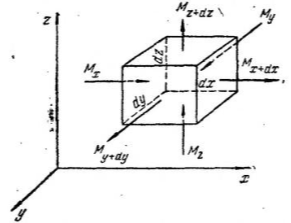
\includegraphics{to_the_conclusion_of_the_differential_equation_of_continuity_of_the_flow.png}
			\caption{К выводу дифференциального уравнения неразрывности потока}
			\label{to_the_conclusion_of_the_differential_equation_of_continuity_of_the_flow}
		\end{center}
	\end{figure}
	\par Пусть составляющая скорости потока вдоль оси \( x \) в точках, лежащих на левой грани параллелепипеда площадью \( dS = dydz \), равна, \( \omega_x \). Тогда, согласно уравнению \( M = \rho \omega S \), через эту грань в параллелепипед войдет вдоль оси \( x \) за единицу времени масса жидкости \( \rho \omega_x dydz \), а за промежуток времени \( d\tau \) - масса жидкости
	\begin{center}
		\( M_x = \rho \omega_x dydzd\tau \)
	\end{center}
	где \( \rho \) - плотность жидкости на левой грани параллелепипеда.
	\par На противоположной (правой) грани параллелепипеда скорость и плотность жидкости могут отличаться от соответствующих величин на левой грани и будут равны \( (\omega_x + \frac{\partial \omega_x}{\partial x} dx) \) и \( (\rho + \frac{\partial \rho}{\partial x} dx)\). Тогда через правую грань параллелепипеда за то же время \( d\tau \) выйдет масса жидкости
	\begin{center}
		\( M_{x+dx} = (\rho \omega_x + \frac{\partial (\rho \omega_x)}{\partial x} dx) dydzd\tau \)
	\end{center}
	\par Приращение массы жидкости в параллелепипеде вдоль оси x:
	\begin{center}
		\( dM_x = M_x - M_{x+dx} = -\frac{\partial (\rho \omega_x)}{\partial x} dxdydzd\tau \)
	\end{center}
	\par Если составляющие скорости вдоль осей \( y \) и \( z \) равны \( \omega_y \) и \( \omega_z \) соответственно, то приращения массы в элементарном объеме вдоль этих осей по аналогии составят:
	\begin{center}
		\( M_y = -\frac{\partial (\rho \omega_y)}{\partial y} dydxdzd\tau \) \\
		\( M_z = -\frac{\partial (\rho \omega_z)}{\partial z} dzdxdyd\tau \)
	\end{center}
	\par Общее накопление массы жидкости в параллелепипеде за время \( d\tau \) равно сумме ее приращений вдоль всех осей координат:
	\begin{center}
		\( dM = - (\frac{\partial (\rho \omega_x)}{\partial x} + \frac{\partial (\rho \omega_y)}{\partial y} + \frac{\partial (\rho \omega_z)}{\partial z}) dxdydzd\tau \)
	\end{center}
	\par Вместе с тем изменение массы в полностью заполненном жидкостью объеме параллелепипеда возможно только вследствие изменения плотности жидкости в этом объеме. Поэтому
	\begin{center}
		\( dM = \frac{\partial \rho}{\partial \tau} dxdydzd\tau \)
	\end{center}
	\par Приравнивая оба выражения \( dM \), сокращая на \( (-dxdydz) \) и перенося \( \frac{\partial \rho}{\partial \tau} \) в левую часть уравнения, окончательно получим
	\begin{center}
		\( \frac{\partial \rho}{\partial \tau} + \frac{\partial (\rho \omega_x)}{\partial x} + \frac{\partial (\rho \omega_y)}{\partial y} + \frac{\partial (\rho \omega_z)}{\partial z} = 0 \)
	\end{center}
	\par Уравнение представляет собой \textit{дифференциальное уравнение неразрывности потока для неустановившегося движения сжимаемой жидкости}.
	\par В установившемся потоке плотность не изменяется во времени, т.е. \( \frac{\partial \rho}{\partial \tau} = 0 \), и уравнение принимает вид
	\begin{center}
		\( \frac{\partial (\rho \omega_x)}{\partial x} + \frac{\partial (\rho \omega_y)}{\partial y} + \frac{\partial (\rho \omega_z)}{\partial z} = 0 \)
	\end{center}
	\par Для капельных жидкостей, которые практически несжимаемы, а также для газов в условиях изотермического потока при скоростях, значительно меньших скорости звука, \( p = const \) и, следовательно
	\begin{center}
		\( \frac{\partial \omega_x}{\partial x} + \frac{\partial \omega_y}{\partial y} + \frac{\partial \omega_z}{\partial z} = 0 \)
	\end{center}
	\par Уравнение является \textit{дифференциальным уравнением неразрывности потока несжимаемой жидкости}.

	\subsubsection{Вывод уравнения Навье-Стокса для одномерного движения. Каков физический смысл слагаемых?}
	\begin{center}
		\underline{Ответ}
	\end{center}
	\par При движении реальной (вязкой) жидкости в потоке жидкости помимо сил давления и тяжести действуют также силы трения.
	\par Действие сил трения \( T \) на выделенный в потоке вязкой жидкости элементарный параллелепипед (рис. \ref{to_derive_the_Navier-Stokes_equations}) проявляется в возникновении на его поверхности касательных напряжений \( \tau \). Рассмотрим первоначально относительно простой случай \textit{одномерного} плоского потока \textit{капельной} жидкости в направлении оси \( x \), когда проекция скорости \( \omega_x \) зависит только от расстояния \( z \) до горизонтальной плоскости отсчета.
	\begin{figure}[H]
		\begin{center}
			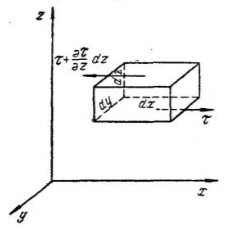
\includegraphics{to_derive_the_Navier-Stokes_equations.png}
			\caption{К выводу уравнений Навье-Стокса}
			\label{to_derive_the_Navier-Stokes_equations}
		\end{center}
	\end{figure}
	\par В этих условиях касательные напряжения возникают лишь на поверхностях \( dF \) верхней и нижней граней элементарного параллелепипеда, причем \( dF = dxdy \). Если касательное напряжение на нижней грани параллелепипеда равно \( \tau \), то на верхней оно составляет \( \tau + \frac{\partial \tau}{\partial z} dz \). Производная \( \frac{\partial \tau}{\partial z} \) выражает изменение касательного напряжения вдоль оси \( z \) в точках, лежащих на нижней грани параллелепипеда, а \( \frac{\partial \tau}{\partial z} dz \) представляет собой изменение этого напряжения вдоль всей длины \( dz \) ребра параллелепипеда.


\end{document}
